\documentclass{beamer}
%
% Choose how your presentation looks.
%
% For more themes, color themes and font themes, see:
% http://deic.uab.es/~iblanes/beamer_gallery/index_by_theme.html
%
\mode<presentation> {
  \usetheme{AnnArbor} % My favorite!
  \setbeamercovered{transparent}
	\setbeamercolor*{palette primary}{use=structure, fg=white, bg=black!50!Purdue-gold}
	\setbeamercolor*{palette secondary}{use=structure, fg=white, bg=Purdue-gold}
	\setbeamercolor*{palette tertiary}{use=structure, fg=white, bg=black}

    \setbeamercolor*{frametitle}{fg=white, bg=Purdue-gold}
    \setbeamercolor{title}{fg=white, bg=Purdue-gold}
	\setbeamercolor{block title}{use=structure, fg=white, bg=Purdue-yellow}
	\setbeamercolor{block body}{use=structure, fg=black, bg=Purdue-yellow!30!white}
    \setbeamercolor{background canvas}{bg=white}
    \setbeamercolor*{item}{use-structure, fg=Purdue-gray}
    
}
\usepackage{color}
\definecolor{Purdue-gold}{RGB}{163, 121, 44}
\definecolor{Purdue-yellow}{RGB}{227, 174, 36}
\definecolor{Purdue-gray}{RGB}{116, 108, 102}

\setbeamertemplate{navigation symbols}{}
\usepackage{amsmath,amsfonts,amsthm,amssymb}
\usepackage{cite}
\usepackage{algorithm2e}
\usepackage{listings}
\usepackage{graphicx}
\usepackage{xcolor}
\usepackage{float}
\usepackage{caption}
\usepackage{subcaption}
\usepackage{multicol}

\usepackage[english]{babel}
\usepackage[utf8x]{inputenc}

\newcommand*\CompactList[0]{
  \vspace*{-3mm}
  \setlength{\itemsep}{0pt}
  \setlength{\parskip}{0pt}
  \setlength{\parsep}{0pt}
}


\title[Bracketology - INFORMS 2014]{Building Perfect Tournament Brackets \newline with Data Analytics}
\author[Hagmann]{Christopher Hagmann, Dr. Nan Kong}
\institute[Purdue]{Purdue University}
\date{November 12, 2014}

\begin{document}

\begin{frame}
  \titlepage
\end{frame}





\section{Introduction}

\begin{frame}{NCAA D-I men's college basketball tournament}
\begin{itemize}
\item Every March, the National Collegiate Athletic Association (NCAA) has collegiate basketball tournaments
\item The most prestigious involve Men's Division I (D-I) \newline "March Madness" tournament
\item Last year, \$1,000,000,000 was offered for correctly predicting \newline all 63 match outcomes
\end{itemize}
\end{frame}

\subsection{Possible Brackets}

\begin{frame}{Distributions of Possible Brackets}
 \begin{figure}[!t]
 \centering
 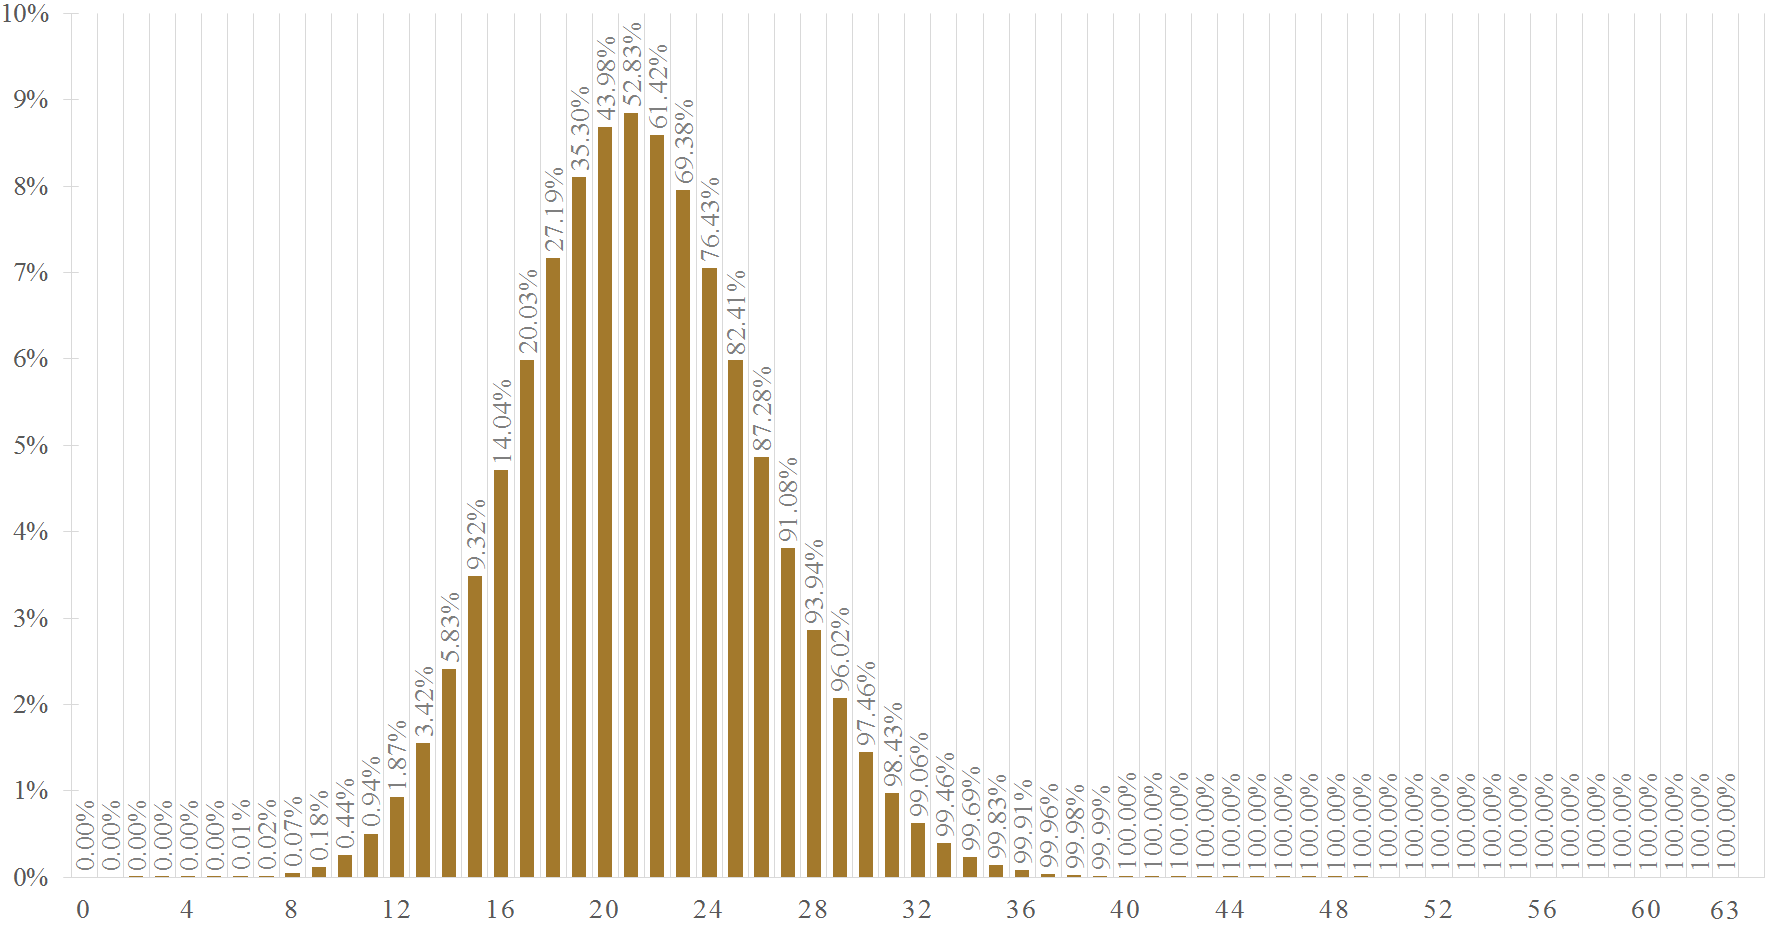
\includegraphics[width=4.75in]{distro.png} 
  \label{distro}
 \end{figure}
\end{frame}


\begin{frame}{Distributions of ESPN Tournament Brackets}
 \begin{figure}[!t]
 \centering
 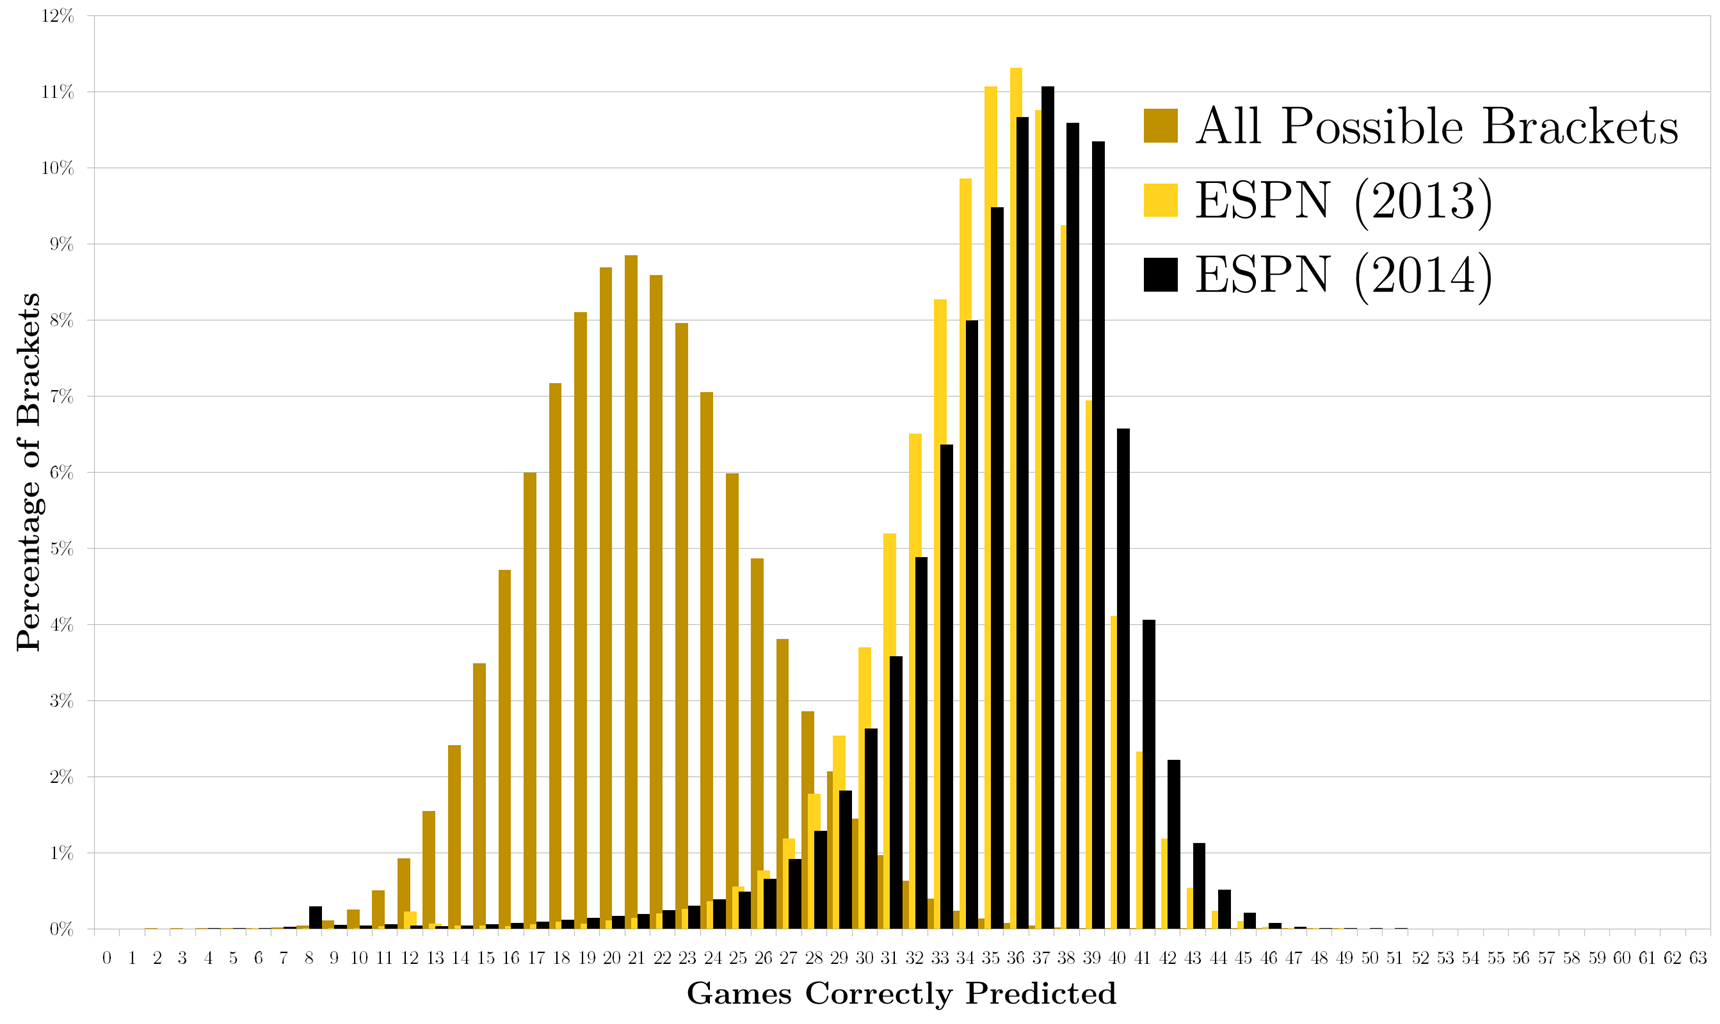
\includegraphics[width=4.75in]{distro2.png} 
  \label{distro}
 \end{figure}
\end{frame}




\subsection{Tempo-Free Statistics}

\begin{frame}{Tempo-Free Statistics}

\begin{itemize}
\item Statistics based on possessions instead of games
\item Allows for better comparisons as the tempo, or number of possessions a team has in a game, varies greatly among players
\end{itemize}
\begin{block}{Example}
Suppose Player A and Player B both average 20 points per game, but the tempo of their respective teams is 60 and 80 possessions per game. This mean Player A is averaging 2 points every 6 possessions while Player B is only averaging 2 points every 8 possessions. Put this way, it is easier to see that Player A is more effective at converting possessions to points than Player B.
\end{block} 
\end{frame}


\begin{frame}{Tempo-Free Statistics}{Definitions}
\begin{block}{Adjusted Offensive Efficiency (AdjO)}
The adjusted offensive efficiency is an estimate of the offensive efficiency (points scored per 100 possessions) a team would have against the \newline average D-I defense.
\end{block}
\begin{block}{Adjusted Defensive Efficiency (AdjD)}
The adjusted defensive efficiency is an estimate of the defensive efficiency (points allowed per 100 possessions) a team would have against the average D-I offense.
\end{block}
\begin{block}{Pythagorean expectation (Pyth)}
The Pythagorean expectation is a descriptive statistic that combines a team's AdjO and AdjD and is an estimate a team’s expected winning percentage against an average D-I team.
\end{block} 
\end{frame}

\begin{frame}{Tempo-Free Statistics}{Ballpark feel}
\huge
\begin{table}[h]
\begin{tabular}{l|c|c|}
\cline{2-3}
                           & Best  & Worse \\ \hline
\multicolumn{1}{|l|}{AdjO} & 125.7 & 97.3  \\ \hline
\multicolumn{1}{|l|}{AdjD} & 86.9  & 108.3 \\ \hline
\multicolumn{1}{|l|}{Pyth} & .9540 & .3552 \\ \hline
\end{tabular}
\end{table}
\end{frame}

\subsection{Current Methods}

\begin{frame}{Picking Chalk}
\begin{block}{Chalk Brackets}
This is a term in sports betting that has its origins back to the days that betting odds were written of chalkboards and refers to always choosing the higher rank team to win. As each team in the tournament bracket is explicitly ranked, using this methods yields a unique bracket that is call the chalk bracket. While this is a very simple idea, it usually fares well in small bracket pools.
\end{block} 
\end{frame}

\begin{frame}{Log5}
Log5 is a method of estimating the probability one team will beat another based on their true winning percentages. In basketball, the Pythagorean expectation is used. It gets its name from it appearance to logit functions and because $p_L \equiv .500$
\[
p_{a,b} = \frac{\frac{p_a}{1-p_a}}{\frac{p_a}{1-p_a} + \frac{p_b}{1-p_b} * \frac{p_L}{1-p_L}} = \frac{p_a (1 - p_b)}{p_a (1 - p_b) + p_b (1 - p_a)}
\]
\end{frame}

\begin{frame}{Log5}
\begin{block}{Notable Properties}
\begin{itemize}
\item If $p_A = 1$, Log5 will always give A a 100\% chance of victory
\item If $p_A = 0$, Log5 will always give A a 0\% chance of victory
\item If $p_A = p_B$, Log5 will always return a 50\% chance of victory for either side
\item If $p_A = 1/2$, Log5 will give A a $1-p_B$ probability of victory.
\end{itemize}
\end{block} 
\end{frame}

\begin{frame}{Interdependence of Games}
There are two ways to look at the likelihood of a team being predicted to advance
\begin{description}
\item[Conditional] Calculate the probability of a team advancing to the next round conditional on all possible games that could occur.
\item[Independent] Calculate the probability based on who is actually in the match, independent of what  has happened or what will happen latter.
\end{description}
\end{frame}



\section{Proposed Method}
\subsection{Overview}

\begin{frame}{Proposed Method}
\begin{itemize}
\item We propose a new method for predicting the perfect bracket.
\item This involve using k-Nearest Neighbor (kNN) to cluster a team's current opponent with their previous opponents to determine a modified winning percentage.
\item This new winning percentage is used in the Log5 to detering the teams odds of winning
\end{itemize}

\end{frame}

\subsection{k-Nearest Neighbor}

\begin{frame}{kNN Algorithm}
  \begin{columns}
    \begin{column}{0.55\textwidth}
\begin{itemize}
\item kNN is a method of regression used to determine a value of a property based on the value of this property in $k$ neighbors
\item The point being examined is a team's current opponent.
\item the possible neighbors are the team's that they have already played
\item The property is the outcome of the game (W/L)
\end{itemize}
    \end{column}


    \begin{column}{0.45\textwidth}
 \begin{figure}[!t]
 \centering
 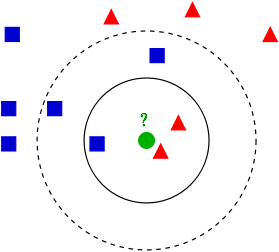
\includegraphics[width=2in]{kNN.png} 
 \end{figure}
\end{column}
\end{columns}

\end{frame}


\subsection{k-Nearest Neighbor}

\begin{frame}{kNN Algorithm}
\begin{itemize}
\item The outcome is weighted based on distance
\item This returns a win and loss score
\item This is repeated for opponent
\item These are aggregated to determine a new winning percentages
\end{itemize}
\[
p_{a} = \frac{W_a + L_b}{W_a + W_b + L_a + L_b}
\]


\end{frame}



\subsection{k-Nearest Neighbor}

\begin{frame}{Finding $k$}
\begin{itemize}
\item The data for the 2003 - 2013 season was provided by Ken Pomeroy and the above methods were applied using $k$ values of between 3 and 25. 25 is the shortest season played, and therefore, the largest neighborhood similar to all teams.
\item It was found that $k=25$ using the conditional method had the highest average number of games corrected predicted, followed by $k=25$ using the independent method. 
\item Second was $k=8$

\end{itemize}



\end{frame}
\section{Results}

\subsection{Note for Comparisons}

\begin{frame}{Note for Comparisons}
\begin{itemize}
\item kNN method performed poorly when compared to standard Log5 method in 2003-2013, average with $k=25$ around 39.5 games correct compared to around 41.1 for Log5. 
\item Parameter in Pythagorean exception was fitted to 2003-2013 data using Log5 as measure.
\item As such 2003-2013 was training set for both.
\item Chalk averaged 40.9 games correct over this time period.

\end{itemize}



\end{frame}

\begin{frame}{Results for 2014 Tournament}

\begin{table}[!t]
 \centering
 \begin{tabular}{|l|c|}
  \hline
  Bracket & Games Correct\\
  \hline
  \hline
  FiveThirtyEight           & 40\\
  Dick Vitale               & 41\\
  President Obama           & 40\\
  "Chalk"                   & 39\\
  Conditional kNN (k=25)*   & 42\\
  Independent kNN (k=25)*   & 40\\
  Log5 (Both Methods)       & 38\\

\hline
\end{tabular}
\caption*{*NOTE: $k=25$ was in fact the best $k$}
\end{table}

\end{frame}

\begin{frame}{Possible Extensions}
\begin{itemize}
\item Add additional attributes in the distance formula
\item Allow for  “upsets”
\item Compare to other regression/classification methods

\end{itemize}
\end{frame}

\section*{Acknowledgment}

\begin{frame}{Acknowledgment}
Special thanks to Ken Pomeroy for providing me with data
\end{frame}

\begin{frame}{Questions?}
\huge
\centerline{Thank You!}
\end{frame}






\end{document}